\chapter{Specifikacija programske potpore}
		
	\section{Funkcionalni zahtjevi}
			
		
			
			
			\noindent \textbf{Dionici:}
			
			\begin{packed_enum}
				
				\item Korisnici aplikacije
				\item Klijenti aplikacije				
				\item Zaposlenici aplikacije
					\begin{packed_enum}
					
					\item Trener
					\item Članovi uprave
					\end{packed_enum}
				\item Administrator
				\item Razvojni tim
				
				
			\end{packed_enum}
			
			\noindent \textbf{Aktori i njihovi funkcionalni zahtjevi:}
			
			
			\begin{packed_enum}
				\item  \underbar{Neregistrirani/neprijavljeni korisnik(inicijator) može:}
				
				\begin{packed_enum}
					
					\item pregledavati sadržaj web aplikacije
					\item dodavati artikle u košaricu web shop-a, brisati jedan ili sve, pregledavati košaricu
					\item registrirati se, tj. napraviti novi korisnički račun s potrebnim podacima
					\item promijeniti jezik aplikacije				
				\end{packed_enum}
			
				\item  \underbar{Klijent (inicijator) aplikacije može:}
				
				\begin{packed_enum}
					
					\item sve što može neregistrirani korisnik osim registracije
					\item pregledavati i mijenjati osobne podatke
					\item izbrisati svoj korisnički račun
					\item platiti narudžbu
					\item ostaviti recenziju na web shop-u
					\item koristiti prijenos utakmica uživo
					\item koristiti chat uslugu pri gledanju prijenosa uživo
					
				\end{packed_enum}
			\pagebreak
			\item  \underbar{Trener, odnosno upravitelj kluba (inicijator) može:}
			
			\begin{packed_enum}
				
				\item dodavati sadržaj na stranicu, brisati ili mijenjati postojeći
				\item dodati novog igrača
				\item promijeniti podatke postojećem igraču
				\item izbrisati igrača iz kluba
				
			\end{packed_enum}
		\item  \underbar{Član uprave (inicijator) može:}
		
		\begin{packed_enum}
			
			\item pregledati aktivne narudžbe
			\item označiti narudžbu zaprimljenom
			\item uređivati artikle na web shop-u
			\item dodati artikl u web shop
			\item dodati popuste na web shop
			
		\end{packed_enum}
	
	\item  \underbar{Administrator aplikacije (inicijator) može:}
	
	\begin{packed_enum}
		
		\item dodavati nove račune (trenera, administratora i upravu)
		\item brisati račune
		\item brisati recenzije
		\item pregledavati klijente
		\item promijeniti prava pristupa
	
	\end{packed_enum}
\item  \underbar{Baza podataka (sudionik):}

\begin{packed_enum}
	
	\item pohranjuje sve podatke o korisnicima i njihovim ovlastima
	\item pohranjuje sve podatke o sadržaju, ponudi i količinama

	
\end{packed_enum}
		\item  \underbar{Banka (sudionik):}
		
		\begin{packed_enum}
			
			\item provjerava, odnosno vrši transakcije prilikom plaćanja u web shop-u
			
			
		\end{packed_enum}
	
		\item  \underbar{YouTube (sudionik):}
		
		\begin{packed_enum}
			\item pruža sučelje za dohvaćanje prijenosa utakmice uživo
		\end{packed_enum}
		
			\end{packed_enum}
			
			\eject 
			
			
				
			\subsection{Obrasci uporabe}
				
				\vspace{20px}
				\textbf{Opis obrazaca uporabe}

				
				\noindent \underbar{\textbf{UC1: Pregled web stranice}}
				\begin{packed_item}
					
					\item \textbf{Glavni sudionik: } Korisnik, klijent
					\item  \textbf{Cilj:} Pregledati sadržaj web stranice, uključujući web shop
					\item  \textbf{Sudionici:} Baza podataka
					\item  \textbf{Preduvjet:}  - 
					\item  \textbf{Opis osnovnog tijeka:}
					
					\item[] \begin{packed_enum}
						\item Stranica je prikazana prilikom pokretanja aplikacije
						\item Korisnik/klijent pregledava sadržaj (Kontakt, O nama, …) 
					\end{packed_enum}
				\end{packed_item}
				
				\vspace{10px}
				
				\noindent \underbar{\textbf{UC2: Registracija}}
				\begin{packed_item}
					
					\item \textbf{Glavni sudionik: } Korisnik
					\item  \textbf{Cilj:} Stvoriti korisnički račun
					\item  \textbf{Sudionici:} Baza podataka
					\item  \textbf{Preduvjet:} - 
					\item  \textbf{Opis osnovnog tijeka:}
					
					\item[] \begin{packed_enum}
						\item Korisnik odabire opciju za registraciju
						\item Korisnik unosi podatke potrebne za registraciju
						\item Korisnik dobiva obavijest o uspješnoj registraciji
					\end{packed_enum}
					\item  \textbf{Opis mogućih odstupanja:}
					\item[] \begin{packed_item}
						
						
						
						\item[2.a]      Odabir već zauzetog korisničkog imena i/ili e-maila, unos korisničkog podatka u nedozvoljenom formatu ili pružanje neispravnoga e-maila
						\item[] \begin{packed_enum}
							\item         Sustav obavještava korisnika o neuspjelom upisu
							\item         Korisnik mijenja potrebne podatke te završava unos ili odustaje od registracije
						\end{packed_enum}
					\end{packed_item}
				\end{packed_item}
				
				\pagebreak
				
				\noindent \underbar{\textbf{UC3: Prijava u sustav}}
				\begin{packed_item}
					
					\item \textbf{Glavni sudionik: } Klijent
					\item  \textbf{Cilj:} Dobiti pristup sustavu
					\item  \textbf{Sudionici:} Baza podataka
					\item  \textbf{Preduvjet:}  Registracija
					\item  \textbf{Opis osnovnog tijeka:}
					
					\item[] \begin{packed_enum}
						\item Korisnik odabire opciju za prijavu
						\item Korisnik unosi podatke potrebne za prijavu (korisničko ime i lozinka)
						\item Korisnik dobiva pristup korisničkim funkcijama
					\end{packed_enum}
					\item  \textbf{Opis mogućih odstupanja:}
					\item[] \begin{packed_item}
						\item[2.a]     Neispravno korisničko ime/lozinka
						\item[] \begin{packed_enum}
							\item          Sustav obavještava korisnika o neuspjelom upisu
						\end{packed_enum}
					\end{packed_item}
				\end{packed_item}
			
				\vspace{10px}
				
				\noindent \underbar{\textbf{UC4: Odjava iz sustava}}
				\begin{packed_item}
					
					\item \textbf{Glavni sudionik: } Klijent
					\item  \textbf{Cilj:} Odjaviti prijavljenog klijenta
					\item  \textbf{Sudionici:} Baza podataka
					\item  \textbf{Preduvjet:}  Prijava u sustav
					\item  \textbf{Opis osnovnog tijeka:}
					
					\item[] \begin{packed_enum}
						\item Klijent odabire opciju za odjavu
						\item Klijent je odjavljen iz sustava i postaje korisnik
					\end{packed_enum}
				\end{packed_item}
				
				\vspace{10px}
				
				\noindent \underbar{\textbf{UC5: Pregled osobnih podataka}}
				\begin{packed_item}
					
					\item \textbf{Glavni sudionik: } Klijent
					\item  \textbf{Cilj:} Pregledati osobne podatke
					\item  \textbf{Sudionici:} Baza podataka
					\item  \textbf{Preduvjet:}  Prijava u sustav
					\item  \textbf{Opis osnovnog tijeka:}
					
					\item[] \begin{packed_enum}
						\item Odabir opcije “Pregled osobnih podataka”
						\item Aplikacija nudi prikaz osobnih podataka
					\end{packed_enum}
				\end{packed_item}
				
				\pagebreak
				
				\noindent \underbar{\textbf{UC6: Promjena osobnih podataka}}
				\begin{packed_item}
					
					\item \textbf{Glavni sudionik: } Klijent
					\item  \textbf{Cilj:} Promijeniti osobne podatke
					\item  \textbf{Sudionici:} Baza podataka
					\item  \textbf{Preduvjet:} Prijava u sustav
					\item  \textbf{Opis osnovnog tijeka:}
					
					\item[] \begin{packed_enum}
						\item Klijent odabire opciju za promjenu podataka
						\item Klijent unosi podatke koje želi mijenjati
						\item Klijent sprema promjene
						\item Baza ažurira promjene
					\end{packed_enum}
					\item  \textbf{Opis mogućih odstupanja:}
					\item[] \begin{packed_item}
						\item[3.a]      Klijent nije spremio promjene
						\item[] \begin{packed_enum}
							\item         Sustav obavještava korisnika da nije spremio promjene
						\end{packed_enum}
					\end{packed_item}
				\end{packed_item}
				
				\noindent \underbar{\textbf{UC7: Brisanje računa}}
				\begin{packed_item}
					
					\item \textbf{Glavni sudionik: } Klijent
					\item  \textbf{Cilj:} Izbrisati svoj korisnički račun
					\item  \textbf{Sudionici:} Baza podataka
					\item  \textbf{Preduvjet:}  Prijava u sustav
					\item  \textbf{Opis osnovnog tijeka:}
					
					\item[] \begin{packed_enum}
						\item Klijent odabire opciju za pregled podataka
						\item Otvara se pregled podataka
						\item Klijent odabire opciju za brisanje računa
						\item Korisnički račun se izbriše
						\item Otvara se početna stranica koju vidi korisnik
					\end{packed_enum}
				\end{packed_item}
				
				\noindent \underbar{\textbf{UC8: Administratorsko brisanje računa}}
				\begin{packed_item}
					
					\item \textbf{Glavni sudionik: } Administrator
					\item  \textbf{Cilj:} Izbrisati klijentski račun
					\item  \textbf{Sudionici:} Baza podataka
					\item  \textbf{Preduvjet:}  Prijava u sustav
					\item  \textbf{Opis osnovnog tijeka:}
					
					\item[] \begin{packed_enum}
						\item Administrator odabire opciju za pregled svih klijenata
						\item Otvara se pregled svih klijenata
						\item Administrator odabire opciju za brisanje određenog klijenta
						\item Klijentski račun se izbriše
					\end{packed_enum}
				\end{packed_item}
				
				\pagebreak
								
				
				\noindent \underbar{\textbf{UC9: Dodavanje novog računa}}
				\begin{packed_item}
					
					\item \textbf{Glavni sudionik: } Administrator
					\item  \textbf{Cilj:} Dodati račun trenera
					\item  \textbf{Sudionici:} Baza podataka
					\item  \textbf{Preduvjet:}  Prijava administratora u sustav
					\item  \textbf{Opis osnovnog tijeka:}
					
					\item[] \begin{packed_enum}
						\item Administrator odabire opciju za pregled svih klijenata
						\item Otvara se pregled svih klijenata
						\item Administrator odabire opciju za dodavanje računa gdje upiše podatke za stvaranje računa
						\item Račun se doda i na email se pošalju podaci za login
					\end{packed_enum}
				\end{packed_item}
				
				\noindent \underbar{\textbf{UC10: Stavljanje artikla u košaricu}}
				\begin{packed_item}
					
					\item \textbf{Glavni sudionik: } Korisnik, klijent
					\item  \textbf{Cilj:} Odabrati artikl koji želi kupiti i staviti ga u košaricu
					\item  \textbf{Sudionici:} Baza podataka
					\item  \textbf{Preduvjet:}  Prijava u sustav
					\item  \textbf{Opis osnovnog tijeka:}
					
					\item[] \begin{packed_enum}
						\item Korisnik/klijent ulazi u web shop
						\item Otvara se pregled ponude
						\item Korisnik/klijent odabire artikl s veličinom koju želi klikom na “Dodaj u košaricu”
						\item Artikl se dodaje u košaricu
					\end{packed_enum}
					\item  \textbf{Opis mogućih odstupanja:}
					\item[] \begin{packed_item}
						\item[3.a]      Korisnik/klijent odabire veličinu/artikl koji je trenutno nedostupan
						\item[] \begin{packed_enum}
							\item         Sustav obavještava korisnika da veličina trenutno nije dostupna i nudi opciju obavijesti kada artikl bude dostupan
						\end{packed_enum}
					\end{packed_item}
				\end{packed_item}
				
				\pagebreak
				
				
				\noindent \underbar{\textbf{UC11: Brisanje artikla iz košarice}}
				\begin{packed_item}
					
					\item \textbf{Glavni sudionik: } Korisnik, klijent
					\item  \textbf{Cilj:} Izbrisati artikl iz košarice
					\item  \textbf{Sudionici:} Baza podataka
					\item  \textbf{Preduvjet:} Prijava u sustav
					\item  \textbf{Opis osnovnog tijeka:}
					
					\item[] \begin{packed_enum}
						\item Korisnik/klijent odabire opciju za pregled košarice
						\item Otvara se košarica
						\item Korisnik/klijent odabire opciju za brisanje određenog artikla iz košarice
						\item Artikl se izbriše iz košarice
					\end{packed_enum}
				\end{packed_item}
				
				\noindent \underbar{\textbf{UC12: Brisanje svih artikala iz košarice}}
				\begin{packed_item}
					
					\item \textbf{Glavni sudionik: } Korisnik/klijent
					\item  \textbf{Cilj:} Isprazniti košaricu
					\item  \textbf{Sudionici:} Baza podataka
					\item  \textbf{Preduvjet:}  Prijava u sustav
					\item  \textbf{Opis osnovnog tijeka:}
					
					\item[] \begin{packed_enum}
						\item Korisnik/klijent ulazi u web shop
						\item Otvara se pregled ponude
						\item Korisnik/klijent odabire opciju “Pregled košarice”
						\item Prikazuje se pregled košarice
						\item Korisnik/klijent odabire opciju “Isprazni košaricu”
						\item Podaci se ažuriraju
					\end{packed_enum}
				\end{packed_item}
				
				
				\noindent \underbar{\textbf{UC13: Pregled košarice}}
				\begin{packed_item}
					
					\item \textbf{Glavni sudionik: } Korisnik, klijent
					\item  \textbf{Cilj:} Pregledati košaricu
					\item  \textbf{Sudionici:} Baza podataka
					\item  \textbf{Preduvjet:}  Prijava u sustav
					\item  \textbf{Opis osnovnog tijeka:}
					
					\item[] \begin{packed_enum}
						\item Korisnik/klijent ulazi u web shop
						\item Otvara se pregled ponude
						\item Korisnik/klijent odabire opciju “Pregled košarice”
						\item Prikazuje se pregled košarice
					\end{packed_enum}
				\end{packed_item}
			
				\pagebreak
				
				\noindent \underbar{\textbf{UC14: Izmjena količine pojedinog artikla u košarici}}
				\begin{packed_item}
					
					\item \textbf{Glavni sudionik: } Korisnik, klijent
					\item  \textbf{Cilj:} Izmijeniti artikle u košarici
					\item  \textbf{Sudionici:} Baza podataka
					\item  \textbf{Preduvjet:}  Prijava u sustav
					\item  \textbf{Opis osnovnog tijeka:}
					
					\item[] \begin{packed_enum}
						\item Korisnik/klijent ulazi u web shop
						\item Otvara se pregled ponude
						\item Korisnik/klijent odabire opciju “Pregled košarice”
						\item Prikazuje se pregled košarice
						\item Korisnik/klijent klikom na “-“ ili “+” upravlja izmjenom količine odabranih artikala u košarici
					\end{packed_enum}
				\end{packed_item}
				
				\noindent \underbar{\textbf{UC15: Plaćanje}}
				\begin{packed_item}
					
					\item \textbf{Glavni sudionik: } Klijent
					\item  \textbf{Cilj:} Platiti narudžbu 
					\item  \textbf{Sudionici:} Baza podataka, Banka
					\item  \textbf{Preduvjet:}  Prijava u sustav
					\item  \textbf{Opis osnovnog tijeka:}
					
					\item[] \begin{packed_enum}
						\item Klijent odabire opciju za “Pregled košarice”
						\item Klijent odabire opciju “Plaćanje”
						\item Klijent unosi podatke potrebne za plaćanje (broj kartice) i opcije dostave
						\item Klijent odabire opciju “Dovrši narudžbu”
						\item Sustav komunicira s bankom i vrši transakciju
						\item Sustav pohranjuje podatke o narudžbi te šalje email obavijest o uspješno obavljenoj narudžbi
					\end{packed_enum}
					\item  \textbf{Opis mogućih odstupanja:}
					\item[] \begin{packed_item}
						\item[3.a]      Klijent unosi neispravnu karticu
						\item[] \begin{packed_enum}
							\item         Sustav obavještava korisnika da je broj kartice neispravan te nudi opciju ponovnog upisa ili odustajanja od narudžbe
						\end{packed_enum}
						
						\item[4.a]      Odustajanje od narudžbe
						\item[] \begin{packed_enum}
							\item         Sustav nudi opciju “Jeste li sigurni da želite odustati?”
						\end{packed_enum}
						\item[5.a]  Nedovoljan iznos na računu
						\item[] \begin{packed_enum}
							\item         Sustav obavještava klijenta o tome da transakcija nije mogla biti provedena
						\end{packed_enum}
					\end{packed_item}
				\end{packed_item}
				
				\pagebreak
				
				\noindent \underbar{\textbf{UC16: Recenzija proizvoda}}
				\begin{packed_item}
					
					\item \textbf{Glavni sudionik: } Klijent
					\item  \textbf{Cilj:} Ocijeniti proizvod u web shopu
					\item  \textbf{Sudionici:} Baza podataka
					\item  \textbf{Preduvjet:}  Prijava u sustav, plaćanje proizvoda, potvrda od uprave o dovršenoj narudžbi
					\item  \textbf{Opis osnovnog tijeka:}
					
					\item[] \begin{packed_enum}
						\item Klijent ulazi u web shop
						\item Otvara se pregled ponude
						\item Klijent odabire artikl i opciju “Ostavi recenziju”
						\item Klijent upiše ocjenu i recenziju 
						\item Klijent odabire opciju spremi
						\item Promjene se ažuriraju
					\end{packed_enum}
					\item  \textbf{Opis mogućih odstupanja:}
					\item[] \begin{packed_item}
						\item[5.a]      Klijent nije spremio promjene
						\item[] \begin{packed_enum}
							\item         Sustav obavještava korisnika da nije spremio recenziju
						\end{packed_enum}
					\end{packed_item}
				\end{packed_item}
				
				\vspace{10px}
				
				
				\noindent \underbar{\textbf{UC17: Brisanje recenzije}}
				\begin{packed_item}
					
					\item \textbf{Glavni sudionik: } Administrator
					\item  \textbf{Cilj:} Obrisati recenziju
					\item  \textbf{Sudionici:} Baza podataka
					\item  \textbf{Preduvjet:} Administrator je prijavljen na sustav
					\item  \textbf{Opis osnovnog tijeka:}
					
					\item[] \begin{packed_enum}
						\item Administrator pronalazi željenu recenziju i odabire opciju “Obriši”
						\item Ažuriraju se promjene
					\end{packed_enum}
				\end{packed_item}
			
				\pagebreak
				
				\noindent \underbar{\textbf{UC18: Pregled aktivnih narudžbi}}
				\begin{packed_item}
					
					\item \textbf{Glavni sudionik: } Uprava
					\item  \textbf{Cilj:} Pregledati aktivne narudžbe
					\item  \textbf{Sudionici:} Baza podataka
					\item  \textbf{Preduvjet:} Uprava je prijavljena u sustav, narudžba je zaprimljena i plaćena
					\item  \textbf{Opis osnovnog tijeka:}
					
					\item[] \begin{packed_enum}
						\item Uprava odabire opciju “Aktivne narudžbe”
						\item Prikazuju se aktivne narudžbe
					\end{packed_enum}
				\end{packed_item}
				
				\noindent \underbar{\textbf{UC19: Označavanje narudžbe zaprimljenom}}
				\begin{packed_item}
					
					\item \textbf{Glavni sudionik: } Uprava
					\item  \textbf{Cilj:} Označiti narudžbu zaprimljenom
					\item  \textbf{Sudionici:} Baza podataka, klijent
					\item  \textbf{Preduvjet:}  Uprava je prijavljena u sustav, narudžba je zaprimljena i plaćena
					\item  \textbf{Opis osnovnog tijeka:}
					
					\item[] \begin{packed_enum}
						\item Uprava pregledava aktivne narudžbe
						\item Uprava odabire narudžbu i označi ju zaprimljenom
						\item Klijentu se šalje obavijest
					\end{packed_enum}
				\end{packed_item}
				
				\noindent \underbar{\textbf{UC20: Dodavanje artikla u web shop}}
				\begin{packed_item}
					
					\item \textbf{Glavni sudionik: } Uprava
					\item  \textbf{Cilj:} Dodati artikl u web shop
					\item  \textbf{Sudionici:} Baza podataka
					\item  \textbf{Preduvjet:}  Uprava je prijavljena u sustav
					\item  \textbf{Opis osnovnog tijeka:}
					
					\item[] \begin{packed_enum}
						\item Uprava pregledava web shop
						\item Uprava odabere opciju “Dodaj artikl”
						\item Uprava ispunjava podatke vezane uz artikl 
						\item Promjene se upisuju u bazu podataka
						\item Slanje e-mail obavijesti korisnicima
					\end{packed_enum}
				\end{packed_item}
				
				\pagebreak
				
				\noindent \underbar{\textbf{UC21: Uređivanje artikala u web shopu}}
				\begin{packed_item}
					
					\item \textbf{Glavni sudionik: } Uprava
					\item  \textbf{Cilj:} Promijeniti sadržaj artikala
					\item  \textbf{Sudionici:} Baza podataka
					\item  \textbf{Preduvjet:} Uprava je prijavljena u sustav
					\item  \textbf{Opis osnovnog tijeka:}
					
					\item[] \begin{packed_enum}
						\item Uprava pregledava web shop
						\item Uprava odabire opciju “Promijeni podatke” odabranom artiklu 
						\item Uprava ispunjava podatke vezane uz podatke
						\item Promjene se upisuju u bazu podataka
						\item Slanje obavijesti korisnicima
					\end{packed_enum}
				\end{packed_item}
			
				
				\noindent \underbar{\textbf{UC22: Dodavanje popusta na web shop}}
				\begin{packed_item}
					
					\item \textbf{Glavni sudionik: } Uprava
					\item  \textbf{Cilj:} Dodati popust u web shop
					\item  \textbf{Sudionici:} Baza podataka
					\item  \textbf{Preduvjet:} Uprava je prijavljena u sustav
					\item  \textbf{Opis osnovnog tijeka:}
					
					\item[] \begin{packed_enum}
						\item Uprava pregledava web shop
						\item Uprava odabire opciju “Dodaj popust”
						\item Uprava ispunjava podatke vezane uz popust
						\item Promjene se upisuju u bazu podataka
						\item Slanje obavijesti korisnicima
					\end{packed_enum}
				\end{packed_item}
				
				
				\noindent \underbar{\textbf{UC23: Dodavanje novog igrača}}
				\begin{packed_item}
					
					\item \textbf{Glavni sudionik: } Trener
					\item  \textbf{Cilj:} Dodati novog igrača u tim
					\item  \textbf{Sudionici:} Baza podataka
					\item  \textbf{Preduvjet:}  Trener je prijavljena u sustav
					\item  \textbf{Opis osnovnog tijeka:}
					
					\item[] \begin{packed_enum}
						\item Trener pregledava sadržaj
						\item Trener odabere opciju “Dodaj novog igrača”
						\item Trener upisuje podatke o novom igraču i odabere opciju za spremanje podataka
						\item  Promjene se upisuju u bazu podataka
					\end{packed_enum}
				\end{packed_item}
				
				\pagebreak
				
				
				\noindent \underbar{\textbf{UC24: Promjena podataka postojećem igraču}}
				\begin{packed_item}
					
					\item \textbf{Glavni sudionik: } Trener
					\item  \textbf{Cilj:} Promijeniti podatke postojećem igraču
					\item  \textbf{Sudionici:} Baza podataka
					\item  \textbf{Preduvjet:} Trener je prijavljena u sustav
					\item  \textbf{Opis osnovnog tijeka:}
					
					\item[] \begin{packed_enum}
						\item Trener pregledava igrače
						\item Trener odabere opciju “Promijeni podatke igrača”
						\item Trener upisuje novi sadržaj i odabere opciju za spremanje podataka
						\item  Promjene se upisuju u bazu podataka
					\end{packed_enum}
				\end{packed_item}
				
				
				\noindent \underbar{\textbf{UC25: Brisanje igrača}}
				\begin{packed_item}
					
					\item \textbf{Glavni sudionik: } Trener
					\item  \textbf{Cilj:} Izbrisati igrača iz tima
					\item  \textbf{Sudionici:} Baza podataka
					\item  \textbf{Preduvjet:} Trener je prijavljena u sustav
					\item  \textbf{Opis osnovnog tijeka:}
					
					\item[] \begin{packed_enum}
						\item Trener pregledava igrače
						\item Trener odabere opciju “Izbriši igrača”
						\item  Promjene se upisuju u bazu podataka
					\end{packed_enum}
				\end{packed_item}
				
				\noindent \underbar{\textbf{UC26: Dodavanje novog sadržaja}}
				\begin{packed_item}
					
					\item \textbf{Glavni sudionik: } Trener
					\item  \textbf{Cilj:} Dodati novi tekstualni sadržaj/sliku
					\item  \textbf{Sudionici:} Baza podataka
					\item  \textbf{Preduvjet:} Trener je prijavljen u sustav
					\item  \textbf{Opis osnovnog tijeka:}
					
					\item[] \begin{packed_enum}
						\item Trener pregledava sadržaj
						\item Trener odabere opciju “Dodaj novi sadržaj”
						\item Trener upisuje novi sadržaj i odabire opciju za spremanje podataka
						\item  Promjene se upisuju u bazu podataka
					\end{packed_enum}
				\end{packed_item}
				
				\pagebreak
				
				\noindent \underbar{\textbf{UC27: Uređivanje postojećeg sadržaja}}
				\begin{packed_item}
					
					\item \textbf{Glavni sudionik: } Trener
					\item  \textbf{Cilj:} Promijeniti već postojeći sadržaj
					\item  \textbf{Sudionici:} Baza podataka
					\item  \textbf{Preduvjet:} Trener je prijavljen u sustav
					\item  \textbf{Opis osnovnog tijeka:}
					
					\item[] \begin{packed_enum}
						\item Trener pregledava sadržaj
						\item Trener odabere opciju “Uredi”
						\item Trener ispunjava podatke koje želi izmijeniti
						\item Promjene se upisuju u bazu podataka
					\end{packed_enum}
				\end{packed_item}
				
				
				\noindent \underbar{\textbf{UC28: Brisanje postojećeg sadržaja}}
				\begin{packed_item}
					
					\item \textbf{Glavni sudionik: } Trener
					\item  \textbf{Cilj:} Obrisati stvoreni sadržaj
					\item  \textbf{Sudionici:} Baza podataka
					\item  \textbf{Preduvjet:} Trener je prijavljen u sustav
					\item  \textbf{Opis osnovnog tijeka:}
					
					\item[] \begin{packed_enum}
						\item Trener pregledava sadržaj
						\item Trener odabere opciju “Obriši”
						\item  Promjene se upisuju u bazu podataka
					\end{packed_enum}
				\end{packed_item}
				
				\noindent \underbar{\textbf{UC29: Promjena jezika aplikacije}}
				\begin{packed_item}
					
					\item \textbf{Glavni sudionik: } Korisnik, klijent
					\item  \textbf{Cilj:} Promijeniti jezik prikazivanja
					\item  \textbf{Sudionici:} Baza podataka
					\item  \textbf{Preduvjet:} -
					\item  \textbf{Opis osnovnog tijeka:}
					
					\item[] \begin{packed_enum}
						\item Korisnik/klijent odabire opciju “Promijeni jezik”
						\item Korisnik/klijent odabire jedan od ponuđenih jezika
						\item Prikazuje se stranica na odabranom jeziku
					\end{packed_enum}
				\end{packed_item}
				
				\pagebreak
				
				
				\noindent \underbar{\textbf{UC30: Pregled klijenata}}
				\begin{packed_item}
					
					\item \textbf{Glavni sudionik: } Administrator
					\item  \textbf{Cilj:} Pregledati registrirane korisnike
					\item  \textbf{Sudionici:} Baza podataka
					\item  \textbf{Preduvjet:} Administrator je prijavljen na sustav
					\item  \textbf{Opis osnovnog tijeka:}
					
					\item[] \begin{packed_enum}
						\item Administrator odabire opciju “Pregled klijenata”
						\item Prikazuje se lista svih registriranih korisnika s osobnim podacima         
					\end{packed_enum}
				\end{packed_item}
				
				\noindent \underbar{\textbf{UC31: Promjena prava pristupa}}
				\begin{packed_item}
					
					\item \textbf{Glavni sudionik: } Administrator
					\item  \textbf{Cilj:} Promijeniti pravo pristupa (klijent, trener, uprava, administrator)
					\item  \textbf{Sudionici:} Baza podataka
					\item  \textbf{Preduvjet:} Administrator je prijavljen na sustav
					\item  \textbf{Opis osnovnog tijeka:}
					
					\item[] \begin{packed_enum}
						\item Administrator pronalazi željenog klijenta
						\item Administrator mu dodjeljuje razinu pristupa
					\end{packed_enum}
				\end{packed_item}
				
				\noindent \underbar{\textbf{UC32: Gledanje utakmica uživo}}
				\begin{packed_item}
					
					\item \textbf{Glavni sudionik: } Klijent
					\item  \textbf{Cilj:} Pogledati prijenos utakmice
					\item  \textbf{Sudionici:} YouTube
					\item  \textbf{Preduvjet:} Korisnik je prijavljen
					\item  \textbf{Opis osnovnog tijeka:}
					
					\item[] \begin{packed_enum}
						\item Klijent pronalazi sekciju “Streaming”
						\item Ako je u tijeku utakmica prikaže se prijenos, inače informacije o budućem prijenosu
					\end{packed_enum}
				\end{packed_item}
				
				\noindent \underbar{\textbf{UC33: Korištenje chat usluge u prijenosu}}
				\begin{packed_item}
					
					\item \textbf{Glavni sudionik: } Klijent
					\item  \textbf{Cilj:} Komunikacija klijenata koji gledaju prijenos utakmice
					\item  \textbf{Sudionici:} Baza podataka
					\item  \textbf{Preduvjet:} Klijent je prijavljen
					\item  \textbf{Opis osnovnog tijeka:}
					
					\item[] \begin{packed_enum}
						\item Klijent u tijeku prijenosa s desne strane pronalazi opciju “Chat”
						\item Klijent ostavlja poruku
						\item Ažuriraju se promjene
					\end{packed_enum}
				\end{packed_item}
				
				
					
				\subsubsection{Dijagrami obrazaca uporabe}
					
				
					
					\begin{figure}[H]
						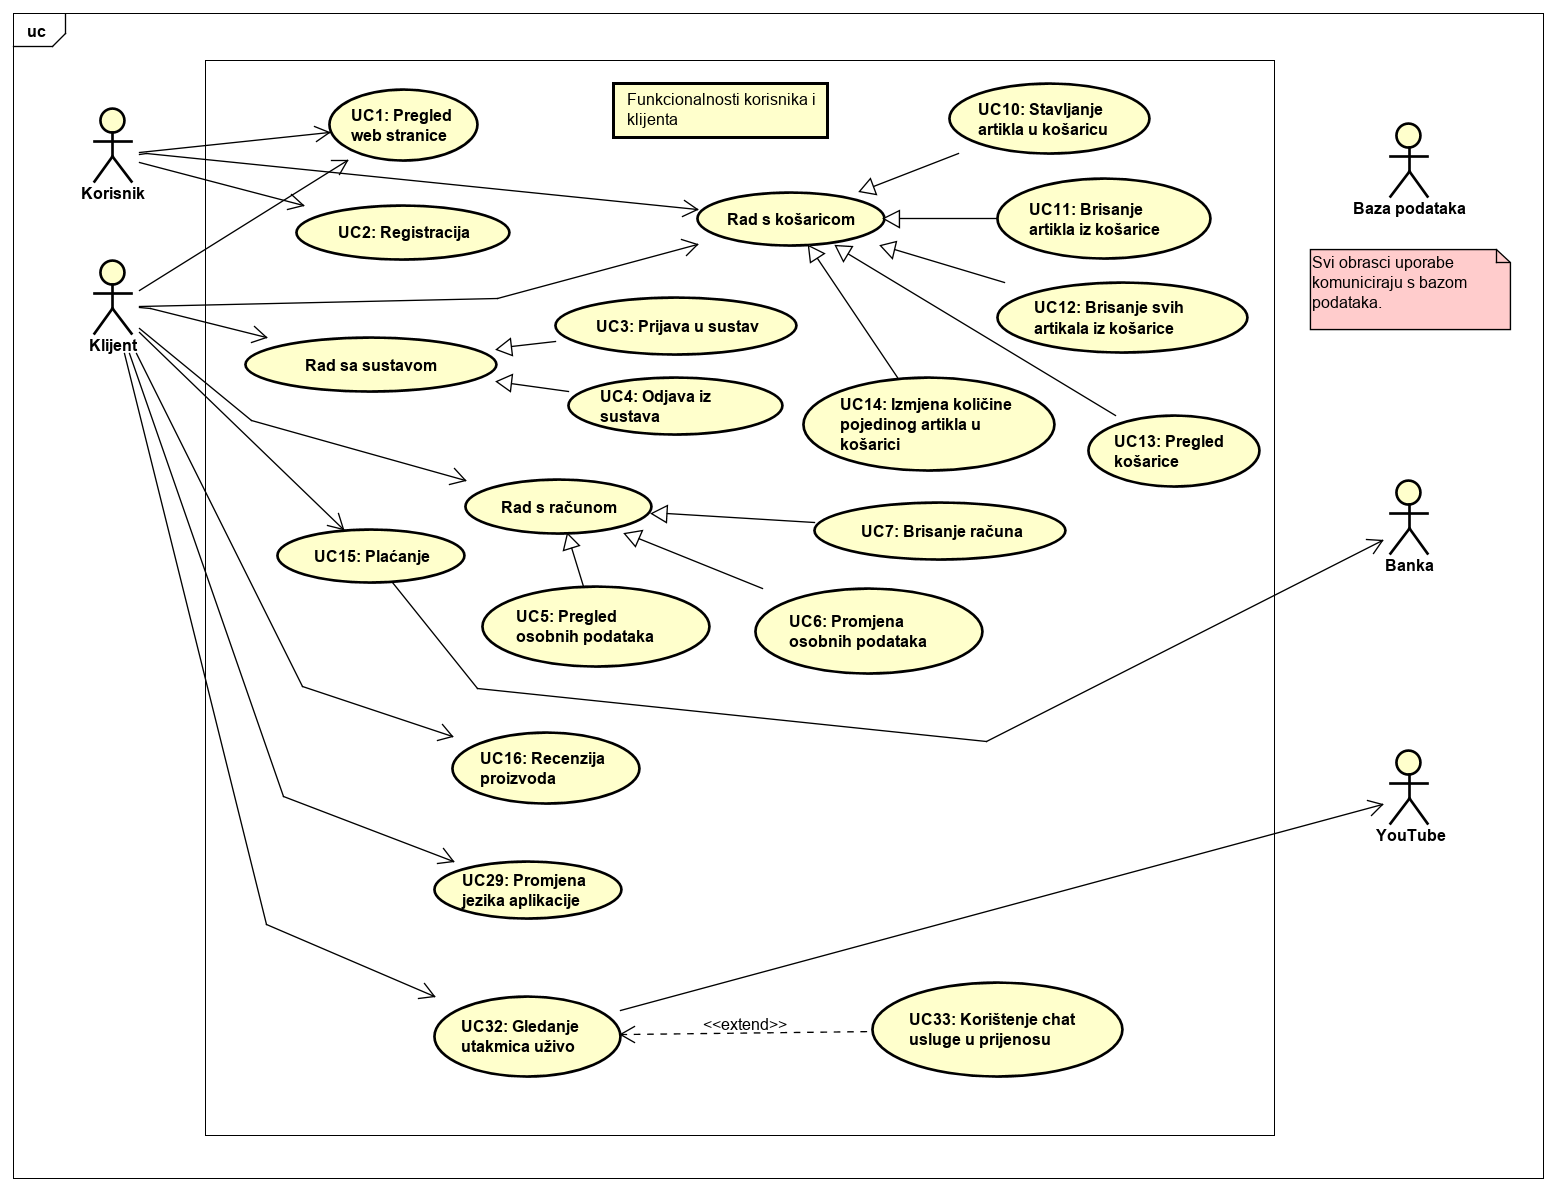
\includegraphics[width=\linewidth]{dijagrami/Funkcionalnosti_korisnika_i_klijenta.png}
						\centering
						\caption{Funkcionalnosti korisnika i klijenta}
						\label{fig:UseCaseDiagram1}
					\end{figure}
				
					\begin{figure}[H]
						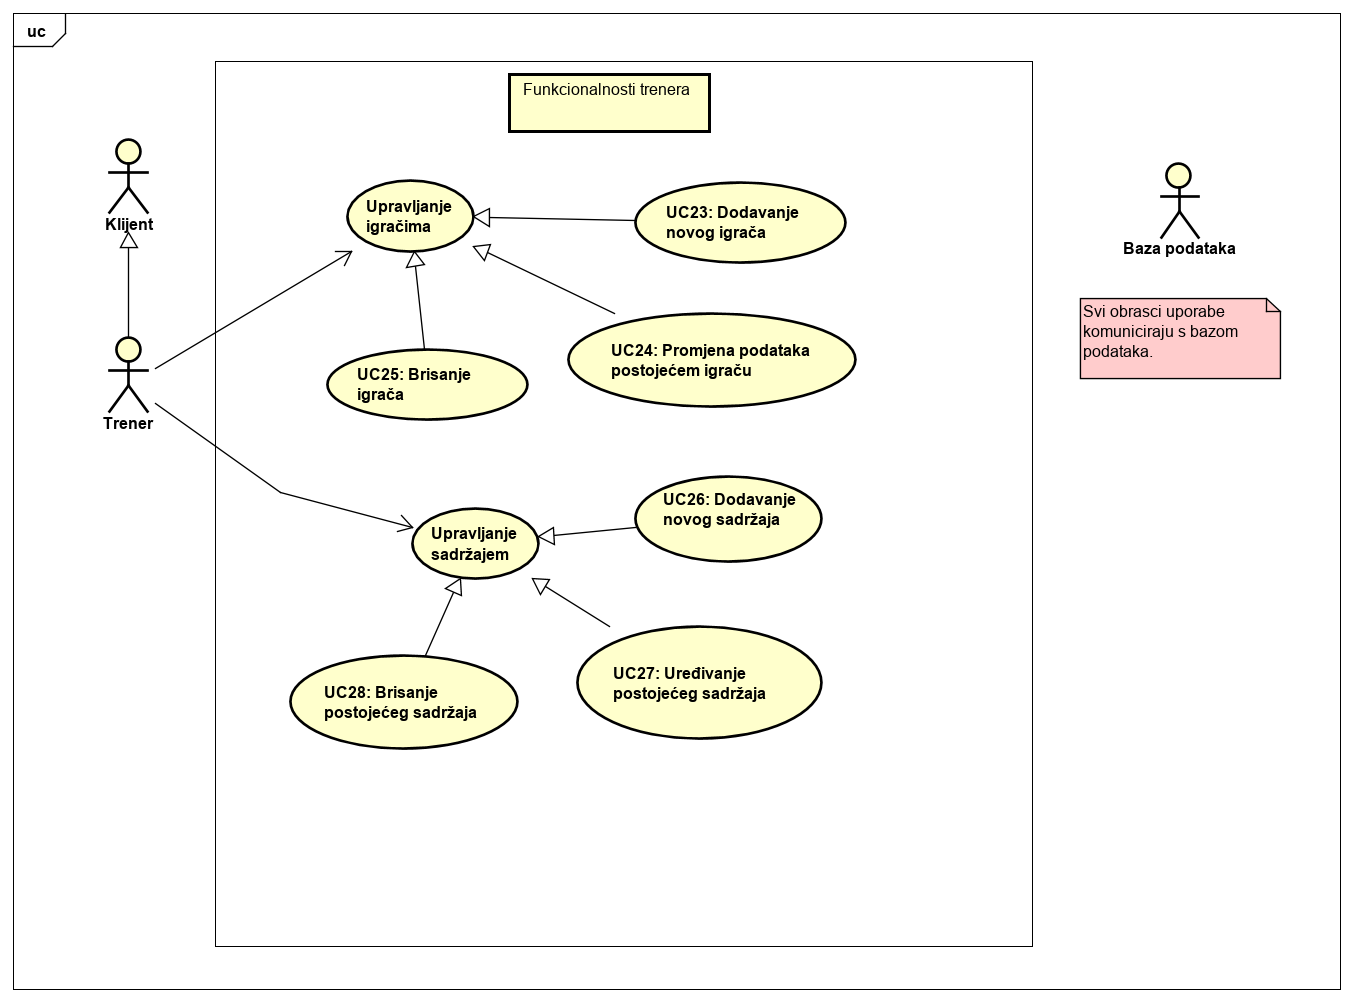
\includegraphics[width=\linewidth]{dijagrami/Funkcionalnosti_trenera.png}
						\centering
						\caption{Funkcionalnosti trenera}
						\label{fig:UseCaseDiagram2}
					\end{figure}
				
					\begin{figure}[H]
						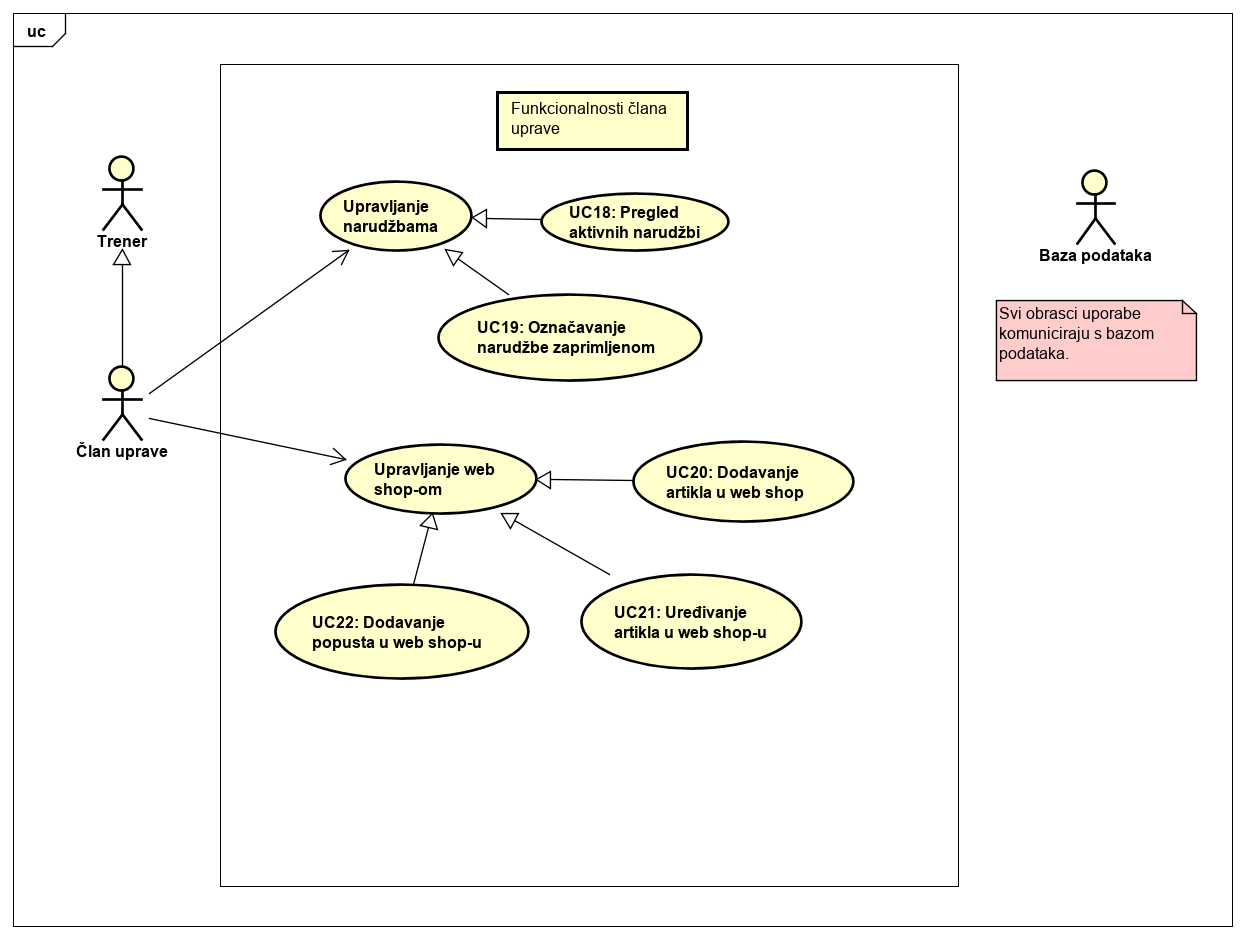
\includegraphics[width=\linewidth]{dijagrami/Funkcionalnosti_clana_uprave.png}
						\centering
						\caption{Funkcionalnosti člana uprave}
						\label{fig:UseCaseDiagram3}
					\end{figure}
				
					\begin{figure}[H]
						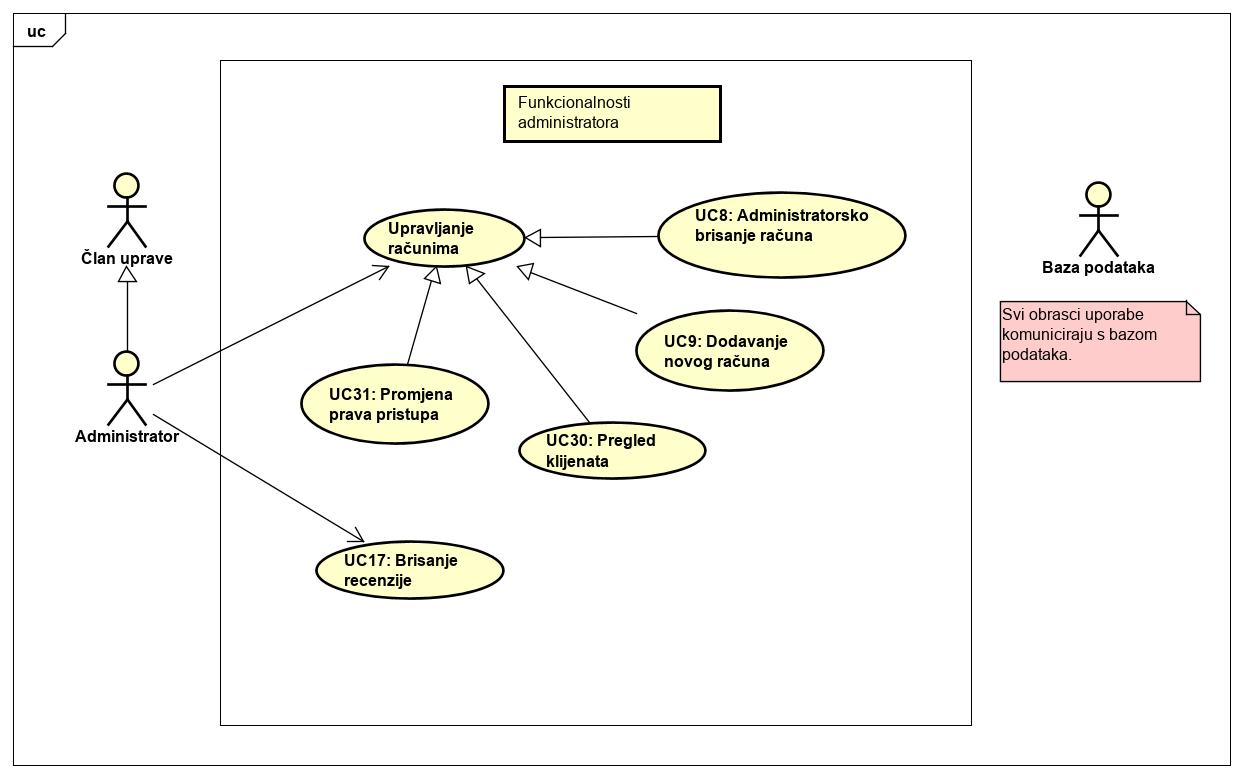
\includegraphics[width=\linewidth]{dijagrami/Funkcionalnosti_administratora.png}
						\centering
						\caption{Funkcionalnosti administratora}
						\label{fig:UseCaseDiagram4}
					\end{figure}
				
				\eject		
				
			\subsection{Sekvencijski dijagrami}
				
				\textbf {Obrazac uporabe UC10: Stavljanje artikla u košaricu }
				\bigbreak
				\textnormal {Korisnik šalje zahtjev za prikaz web shop-a kako bi mogao pregledati artikle. Poslužitelj dohvaća popis artikala i vraća ih te ih prikazuje u web shop-u koji korisnik pregledava. Odabirom artikla, koje korisnik bira dok ne odabere sve željene proizvode, korisnik bira količinu i veličinu proizvoda. Poslužitelj provjerava dostupnost artikla s bazom podataka i vraća informacije o artiklu. Ukoliko je artikl dostupan, korisniku se ispisuje poruka da je artikl dostupan i on šalje zahtjev za dodavanjem u košaricu. Poslužitelj šalje bazi zahtjev za mijenjanje sadržaja košarice, odnosno dodavanja artikla te baza sprema promjene. Ukoliko artikl nije dostupan, korisniku se ispisuje poruka.}
				\begin{figure}[H]
					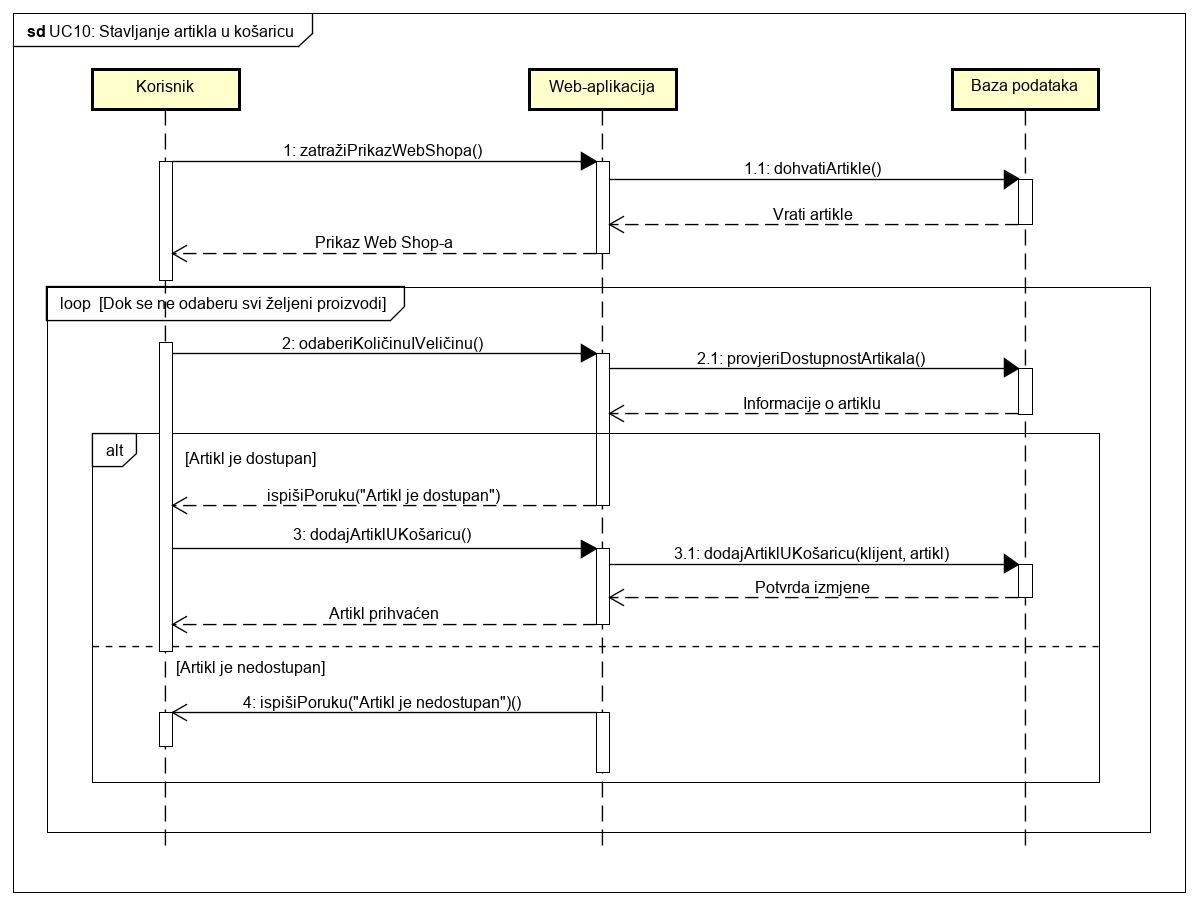
\includegraphics[width=\linewidth]{dijagrami/UC10.png}
					\centering
					\caption{UC10, Stavljanje artikla u košaricu}
					\label{fig:SequanceDiagram1}
				\end{figure}
			\pagebreak
			\textbf {Obrazac uporabe UC15:Plaćanje}
			\bigbreak
			\textnormal {Klijent šalje zahtjev za pregled košarice kako bi mogao vidjeti odabrane artikle u košarici. Poslužitelj dohvaća sadržaj košarice iz baze te ga prikazuje klijentu. Klijent zatraži plaćanje te poslužitelj prikazuje formu za plaćanje koju klijent ispunjava te šalje nazad poslužitelju. Poslužitelj šalje banci zahtjev za transakcijom s određenim iznosom i karticom te banka vraća status transakcije poslužitelju. Na temelju statusa transakcije poslužitelj u bazi formira narudžbu i transakciju te isprazni košaricu. Ukoliko je transakcija odobrena, ispisuje se poruka korisniku. Ukoliko nije, također se ispisuje poruka o neuspješnoj transakciji.}
				\begin{figure}[H]
					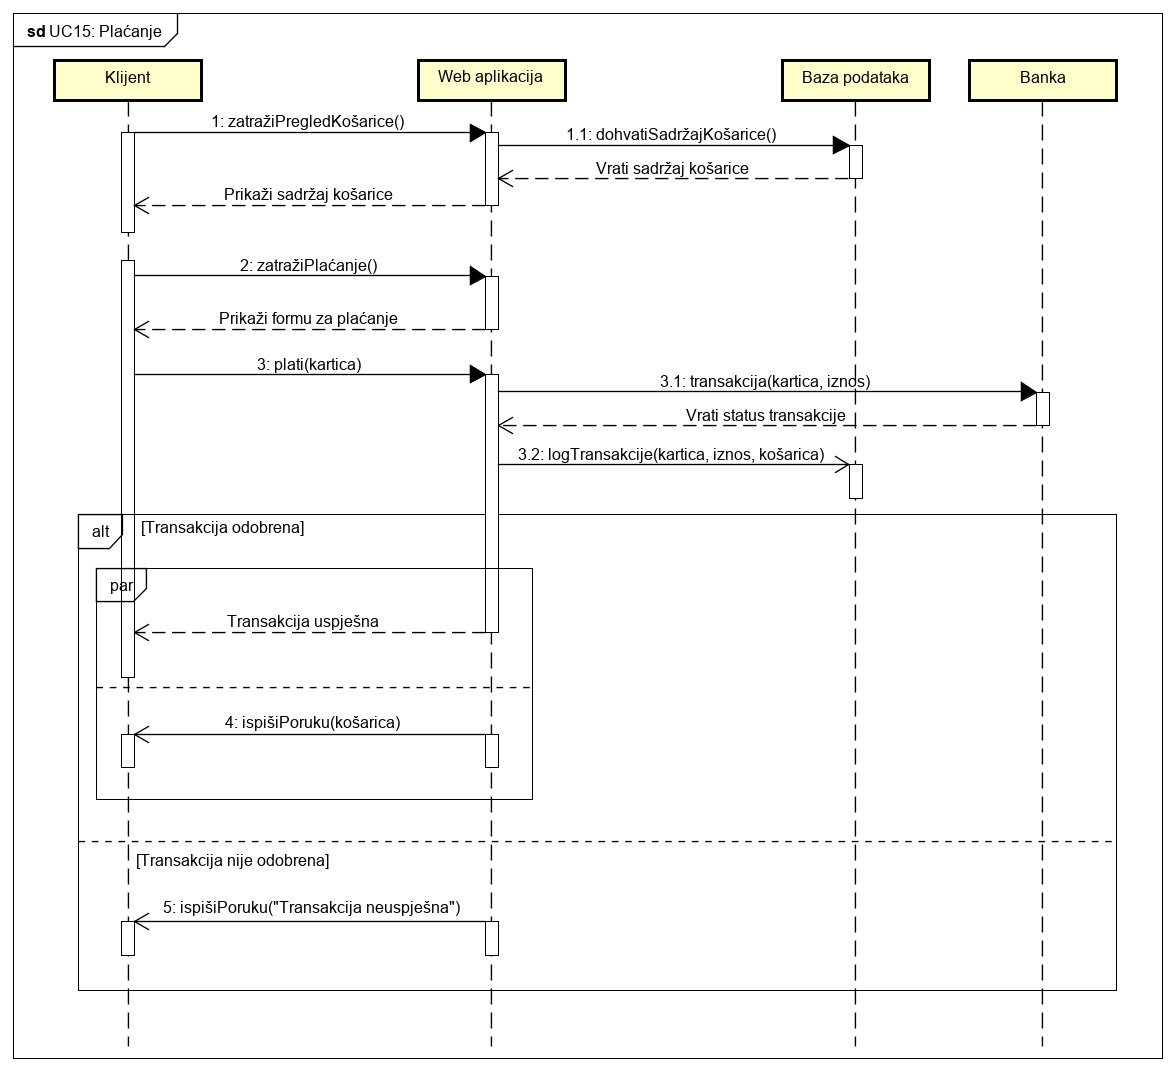
\includegraphics[width=\linewidth]{dijagrami/UC15.png}
					\centering
					\caption{UC15, Plaćanje}
					\label{fig:SequanceDiagram2}
				\end{figure}
			\pagebreak
			\textbf{Obrazac uporabe UC19: Označavanje narudžbe zaprimljenom}
			\bigbreak
			\textnormal {Član uprave zatraži listu aktivnih narudžbi koju poslužitelj proslijeđuje bazi te baza vraća listu aktivnih narudžbi poslužitelju. Ukoliko postoje aktivne narudžbe, poslužitelj ih prikazuje. Dok član uprave ne odabere sve narudžbe koje želi zaprimiti, šalje zahtjev za označavanje narudžbe zaprimljenom poslužitelju koji ih proslijeđuje bazi. Baza zatim potvrđuje izmjene i poslužitelj javlja da su promjene pohranjene. Ukoliko ne postoje aktivne narudžbe, poslužitelj ispisuje odgovarajuću poruku članu uprave.
			}
				\begin{figure}[H]
					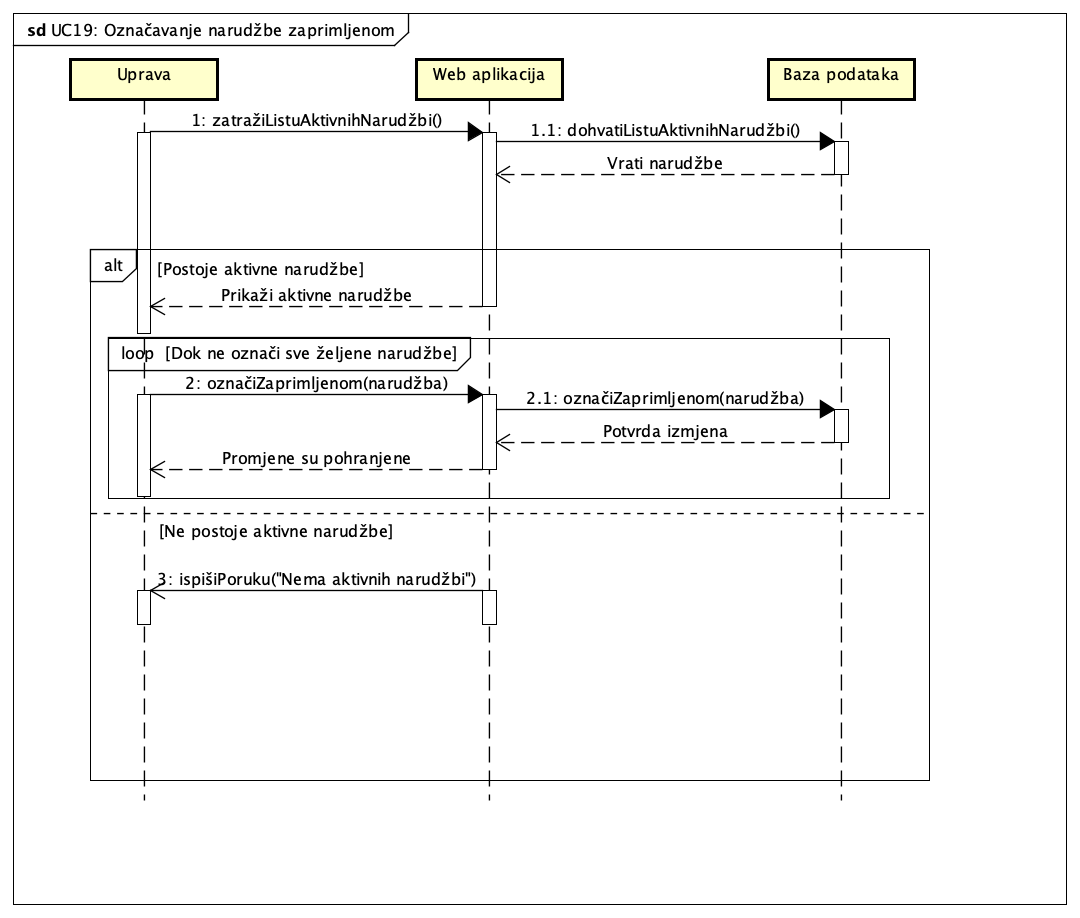
\includegraphics[width=\linewidth]{dijagrami/UC19.png}
					\centering
					\caption{UC19, Označavanje narudžbe gotovom}
					\label{fig:SequanceDiagram3}
				\end{figure}
			\pagebreak
			\textbf{Obrazac uporabe UC21: Uređivanje artikala u web shop-u}
			\bigbreak
			\textnormal {Član uprave šalje zahtjev za prikaz artikala koje poslužitelj dohvaća iz baze te ih prikazuje članu uprave. Član uprave odabere artikl, poslužitelj zatim šalje zahtjev bazi za njegov dohvat te baza vraća artikl koji se prikaže. Član uprave zatraži promjenu proizvoda sa starog na novi te poslužitelj vraća da je pristup odobren. Član uprave šalje promjenu proizvoda koju poslužitelj unosi u bazu podataka koja sprema promjene.}
				\begin{figure}[H]
					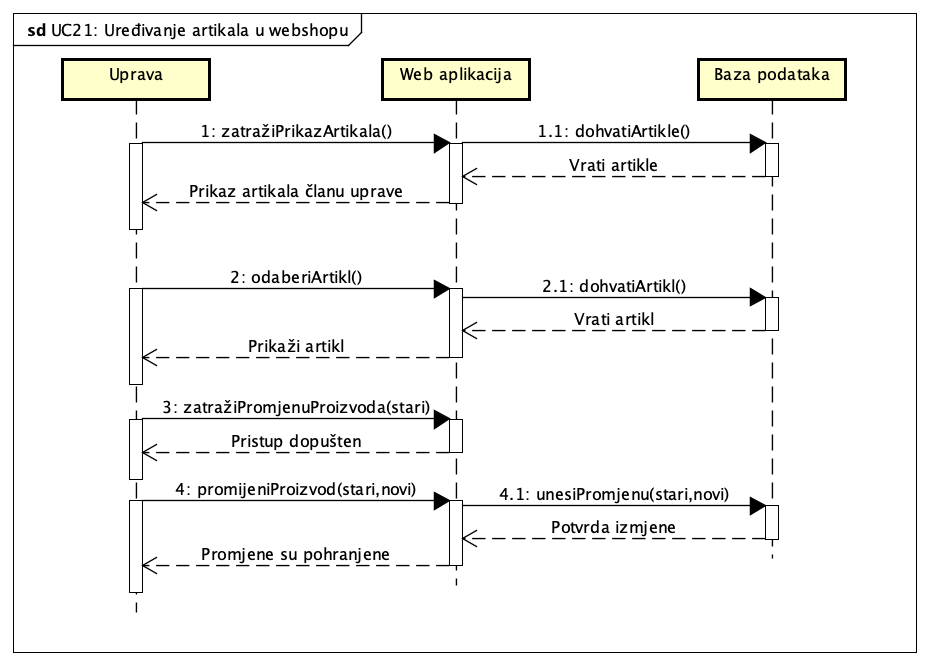
\includegraphics[width=\linewidth]{dijagrami/UC21.png}
					\centering
					\caption{UC21, Uređivanje artikala u web shopu}
					\label{fig:SequanceDiagram4}
				\end{figure}
	\eject
		\section{Ostali zahtjevi}
		
			\begin{packed_item}
				\item Sustav treba omogućiti rad više korisnika u stvarnom vremenu
				\item Korisničko sučelje i sustav moraju podržavati hrvatsku abecedu (dijakritičke znakove) pri unosu i prikazu tekstualnog sadržaja
				\item Izvršavanje dijela programa u kojem se pristupa bazi podataka ne smije trajati duže od nekoliko sekundi
				\item Sustav treba biti implementiran kao web aplikacija koristeći objektno-orijentirane jezike
				\item Neispravno korištenje korisničkog sučelja ne smije narušiti funkcionalnost i rad sustava
				\item Sustav treba biti jednostavan za korištenje, korisnici se moraju znati koristiti sučeljem bez opširnih uputa
				\item Nadogradnja sustava ne smije narušavati postojeće funkcionalnosti sustava
				\item Sustav kao valutu koristi HRK
				\item Veza s bazom podataka mora biti kvalitetno zaštićena, brza i otporna na vanjske greške
				\item Front-end web aplikacije bit će implementiran uz pomoć HTML5, CSS3, Bootstrap 4 i Vue.js tehnologija
				\item Back-end web aplikacije bit će implementiran u programskom jeziku C\#
				\item Čitav sustav će biti utemeljen na okviru rada ASP.NET Core 3.0
				\item Sustav će podržavati hrvatski i engleski jezik
			\end{packed_item}

			 
			 
			 
	